\documentclass[pract,times]{SCWorks}
% Тип обучения (одно из значений):
%    bachelor   - бакалавриат (по умолчанию)
%    spec       - специальность
%    master     - магистратура
% Форма обучения (одно из значений):
%    och        - очное (по умолчанию)
%    zaoch      - заочное
% Тип работы (одно из значений):
%    coursework - курсовая работа (по умолчанию)
%    referat    - реферат
%    otchet     - универсальный отчет
%    nirjournal - журнал НИР
%    diploma    - дипломная работа
%    pract      - отчет о научно-исследовательской работе
%    autoref    - автореферат выпускной работы
%    assignment - задание на выпускную квалификационную работу
%    review     - отзыв руководителя
%    critique   - рецензия на выпускную работу
% Включение шрифта
%    times      - включение шрифта Times New Roman (если установлен)
%                 по умолчанию выключен
\usepackage{preamble}

\begin{document}

% Кафедра (в родительном падеже)
\chair{математической кибернетики и компьютерных наук}

% Тема работы
\title{Теория графов}

% Курс
\course{3}

% Группа
\group{351}

% Факультет (в родительном падеже) (по умолчанию "факультета КНиИТ")
% \department{факультета КНиИТ}

% Специальность/направление код - наименование
% \napravlenie{02.03.02 "--- Фундаментальная информатика и информационные технологии}
% \napravlenie{02.03.01 "--- Математическое обеспечение и администрирование информационных систем}
% \napravlenie{09.03.01 "--- Информатика и вычислительная техника}
\napravlenie{09.03.04 "--- Программная инженерия}
% \napravlenie{10.05.01 "--- Компьютерная безопасность}

% Для студентки. Для работы студента следующая команда не нужна.
% \studenttitle{Студентки}

% Фамилия, имя, отчество в родительном падеже
\author{Мангасаряна Евгения Павловича}

% Заведующий кафедрой
\chtitle{доцент, к.\,ф.-м.\,н.} % степень, звание
\chname{С.\,В.\,Миронов}

% Научный руководитель (для реферата преподаватель проверяющий работу)
\satitle{доцент} %должность, степень, звание
\saname{А.\,П.\,Грецова}

% Семестр (только для практики, для остальных типов работ не используется)
\term{1}

% Наименование практики (только для практики, для остальных типов работ не
% используется)
\practtype{учебная (рассредоточенная)}

% Год выполнения отчета
\date{2023}

\maketitle

% Включение нумерации рисунков, формул и таблиц по разделам (по умолчанию -
% нумерация сквозная) (допускается оба вида нумерации)
\secNumbering

\tableofcontents

\intro
Целью практической работы является закрепление и углубление теоретических знаний по 
дисциплине <<Теория графов>> посредством реализации класса
<<Граф>> на выбранном языке программирования.
Для достижения данной цели были поставлены следующие задачи:
\begin{itemize}
  \item создание класса <<Граф>>;
  \item работа со cписками смежности;
  \item реализация обходов графа;
  \item построение минимального остовного дерева;
  \item работа со взвешенным графом;
  \item реализация потокового алгоритма;
  \item выполнение творческого задания.
\end{itemize}
Все задачи выполнены с использованием языка программирования TypeScript.

\section{Минимальные требования для класса <<Граф>>}
\subsection{Условие задания}
Для решения всех задач курса необходимо создать класс (или иерархию
классов "--- на усмотрение разработчика), содержащий:
\begin{enumerate}
  \item Структуру для хранения списка смежности графа (не работать с графом
  через матрицы смежности, если в некоторых алгоритмах удобнее использовать
  список ребер "--- реализовать метод, создающий список ребер на
  основе списка смежности).
  \item Конструкторы (не менее 3"~х):
  \begin{itemize}
    \item добавляющие вершину;
    \item добавляющие ребро (дугу);
    \item удаляющие вершину;
    \item удаляющие ребро (дугу);
    \item выводящие список смежности в файл (в том числе в пригодном для
    чтения конструктором формате).
  \end{itemize}
  \item Методы:
  \begin{itemize}
    \item конструктор по умолчанию, создающий пустой граф;
    \item конструктор, заполняющий данные графа из файла;
    \item конструктор"=копию (аккуратно, не все сразу делают именно копию);
    \item специфические конструкторы для удобства тестирования.
  \end{itemize}
  \item Должны поддерживаться как ориентированные, так и неориентированные
  графы.
  \item Добавьте минималистичный консольный интерфейс пользователя, позволяющий
  добавлять и удалять вершины и ребра (дуги) и просматривать
  текущий список смежности графа.
\end{enumerate}

\subsection{Примеры исходного кода}
Следующий код описывает класс \mitext{Graph}, соответствующий требованиям
условия:
\begin{minted}{typescript}
export class Graph {
  private adj: Map<string, Map<string, number>> = new Map()
  private weighted: boolean = false
  private oriented: boolean = false

  constructor(weighted: boolean, oriented: boolean)
  constructor(textRepr: string)
  constructor(other: Graph)
  constructor(arg1: boolean | string | Graph, arg2?: boolean) {
    if (typeof arg1 === 'boolean' && typeof arg2 === 'boolean') {
      this.weighted = arg1
      this.oriented = arg2
      this.adj = new Map()
    } else if (typeof arg1 === 'string' && arg2 == null) {
      this.loadFromFile(arg1)
      if (!this.oriented) {
        for (const [v, neighbors] of this.adj) {
          for (const [u, w] of neighbors) {
            this.adj.get(u)!.set(v, w)
          }
        }
      }
    } else if (arg1 instanceof Graph && arg2 == null) {
      this.weighted = arg1.weighted
      this.oriented = arg1.oriented
      this.adj = new Map(arg1.adj)
    } else {
      throw new Error('Invalid arguments')
    }
  }
  // другие методы ...
}
\end{minted}

Методы для добавления вершины и ребра (дуги):
\begin{minted}{typescript}
addNode(label: string) {
  if (this.adj.has(label)) {
    throw new NodeAlreadyExists(label)
  }
  this.adj.set(label, new Map())
}

connect(a: string, b: string, weight?: number) {
  if (!this.adj.has(a)) {
    throw new NodeNotExists(a)
  }
  if (!this.adj.has(b)) {
    throw new NodeNotExists(b)
  }
  if (this.adj.get(a)!.has(b)) {
    throw new ConnectionAlreadyExists(a, b)
  }

  if (this.weighted) {
    this.adj.get(a)!.set(b, weight!)
    if (!this.oriented) {
      this.adj.get(b)!.set(a, weight!)
    }
  } else {
    if (weight) {
      throw new WeightsInNonWeightedGraph()
    }
    this.adj.get(a)!.set(b, 0)
    if (!this.oriented) {
      this.adj.get(b)!.set(a, 0)
    }
  }
}
\end{minted}

Удаление вершины и дуги (ребра):
\begin{minted}{typescript}
removeNode(label: string) {
  if (!this.adj.has(label)) {
    throw new NodeNotExists(label)
  }

  this.adj.delete(label)
  for (let value of this.adj.values()) {
    value.delete(label)
  }
}

disconnect(a: string, b: string) {
  if (!this.adj.has(a)) {
    throw new NodeNotExists(a)
  }
  if (!this.adj.has(b)) {
    throw new NodeNotExists(b)
  }
  if (!this.adj.get(a)!.has(b)) {
    throw new ConnectionNotExists(a, b)
  }

  this.adj.get(a)!.delete(b)
  if (!this.oriented) {
    this.adj.get(b)!.delete(a)
  }
}
\end{minted}

Вместо консольного сразу был реализован веб"=интерфейс на React.js.
Основной компонент интерфейса (\mitext{App}) представлен в приложении
\ref{app:app-component}.

\subsection{Примеры входных и выходных данных}
Взвешенный ориентированный граф:
\begin{minted}{js}
{
  "weighted": true,
  "oriented": true,
  "adj": {
    "a": {
      "b": 2,
      "c": 3
    },
    "b": {
      "d": 5
    },
    "c": {
      "e": 4,
      "f": 2
    },
    "d": {
      "g": 6
    },
    "e": {
      "h": 3
    },
    "f": {
      "h": 7
    },
    "g": {
      "h": 8
    },
    "h": {}
  }
}
\end{minted}

Взвешенный неориентированный граф:
\begin{minted}{js}
{
  "weighted": true,
  "oriented": false,
  "adj": {
    "a": {
      "b": 2,
      "c": 3,
      "d": 5
    },
    "b": {
      "c": 4,
      "e": 6
    },
    "c": {
      "d": 1,
      "f": 3
    },
    "d": {
      "g": 2
    },
    "e": {
      "f": 4,
      "h": 5
    },
    "f": {
      "h": 2,
      "g": 3
    },
    "g": {
      "h": 1
    },
    "h": {}
  }
}
\end{minted}

Выходные файлы имеют такой же формат и полностью совместимы с входными.

\section{Список смежности Ia}
\subsection{Условие задания}
\textbf{Вариант 5:} Для каждой вершины орграфа вывести её степень.

\subsection{Примеры исходного кода}
Для нахождения и вывода степени каждой вершины был создан вспомогательный
компонент \mitext{VertexPowers}, который находит степени вершин и выводит
их в виде таблицы:
\begin{minted}{jsx}
function VertexPowers() {
  const adjList = graph.current!.getAdjacencyList()
  const powers = new Map()

  for (const [k, v] of adjList) {
    powers.set(k, v.length)
    for (const [otherK, otherV] of adjList) {
      if (k === otherK) continue

      if (otherV.find(value => value[0] === k)) {
        powers.set(k, powers.get(k) + 1)
      }
    }
  }

  return (
    <TableBody>
      {graph.current!.getAdjacencyList().map(item => {
        return (
          <TableRow key={item[0]}>
            <TableCell align='right'>{item[0]}</TableCell>
            <TableCell align='left'>{powers.get(item[0])}</TableCell>
          </TableRow>
        )
      })
      }
    </TableBody>
  )
}
\end{minted}

\subsection{Краткое описание алгоритма}
Для каждой вершины подсчитывается степень исхода и степень захода,
а затем суммируются.

\subsection{Примеры входных и выходных данных}
\subsubsection{Входные данные}
\begin{figure}[H]
  \begin{minipage}{0.5\textwidth}
    \centering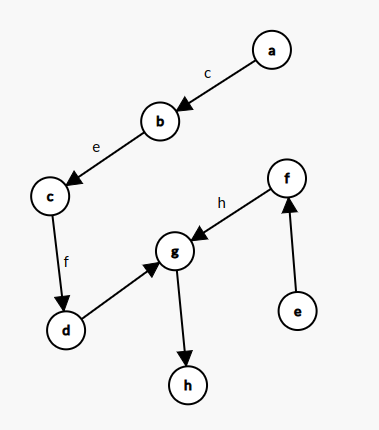
\includegraphics[width=\linewidth]{figs/task-2/graph-1.png}
  \end{minipage}
  \begin{minipage}{0.5\textwidth}
    \centering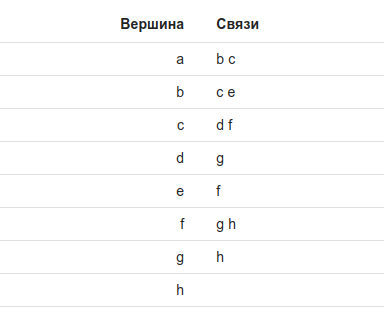
\includegraphics[width=\linewidth]{figs/task-2/adj-1.png}
  \end{minipage}
  \caption{Ориентированный граф}
\end{figure}

\begin{minted}{js}
{
  "weighted": false,
  "oriented": true,
  "adj": {
    "a": {
      "b": 0,
      "c": 0
    },
    "b": {
      "c": 0,
      "e": 0
    },
    "c": {
      "d": 0,
      "f": 0
    },
    "d": {
      "g": 0
    },
    "e": {
      "f": 0
    },
    "f": {
      "g": 0,
      "h": 0
    },
    "g": {
      "h": 0
    },
    "h": {}
  }
}
\end{minted}

\subsubsection{Выходные данные}
\begin{figure}[H]
  \centering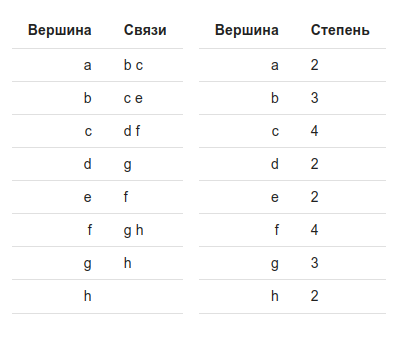
\includegraphics[width=0.5\textwidth]{figs/task-2/res-1.png}
  \caption{Результат работы}
\end{figure}
\section{Список смежности Ia}
\subsection{Условие задания}
\textbf{Вариант 20:} Вывести все вершины орграфа, не смежные с данной.

\subsection{Примеры исходного кода}
Для нахождения и вывода вершин орграфа, не смежных с данной, был
описан метод \mitext{getAdjacent()}:
\begin{minted}{typescript}
getAdjacent(label: string): Map<string, number> {
  if (!this.adj.has(label)) {
    throw new NodeNotExists(label)
  }
  return this.adj.get(label)!
}
\end{minted}

Затем, при выводе результата, запрашиваются все метки вершин орграфа и
из них отбрасываются те, которые смежны с данной:
\begin{minted}{typescript}
let resList: string[] = []
for (const [node, _] of graph.current!.getAdjacencyList()) {
  if (nodeName !== node && !adj.has(node)) {
    resList.push(node.toString())
  }
}
setAnswer(resList.join(', '))
\end{minted}

\subsection{Краткое описание алгоритма}
Поскольку данные о смежности хранятся в виде списка смежности, достаточно
для заданной вершины запросить информацию о смежных с ней вершинах.
А далее простая фильтрация списка строк.

Поскольку графы могут быть взвешенными, и как пересекать веса не оговаривается,
то выбирается минимум из двух весов при пересечении.

\subsection{Примеры входных и выходных данных}
\subsubsection{Входные данные}
\begin{figure}[H]
  \begin{minipage}{0.5\textwidth}
    \centering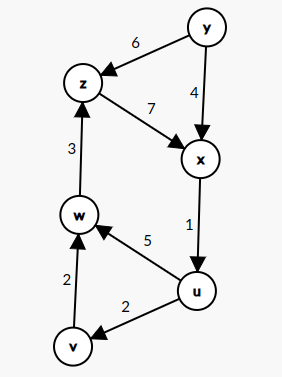
\includegraphics[width=0.6\linewidth]{figs/task-3/graph-2.png}
  \end{minipage}
  \begin{minipage}{0.5\textwidth}
    \centering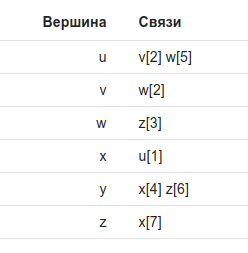
\includegraphics[width=0.6\linewidth]{figs/task-3/adj-2.png}
  \end{minipage}
  \caption{Ориентированный граф}
\end{figure}

\begin{minted}{js}
{
  "weighted": true,
  "oriented": true,
  "adj": {
    "u": {
      "v": 2,
      "w": 5
    },
    "v": {
      "w": 2
    },
    "w": {
      "z": 3
    },
    "x": {
      "u": 1
    },
    "y": {
      "x": 4,
      "z": 6
    },
    "z": {
      "x": 7
    }
  }
}
\end{minted}

\subsubsection{Выходные данные}
\begin{figure}[H]
  \centering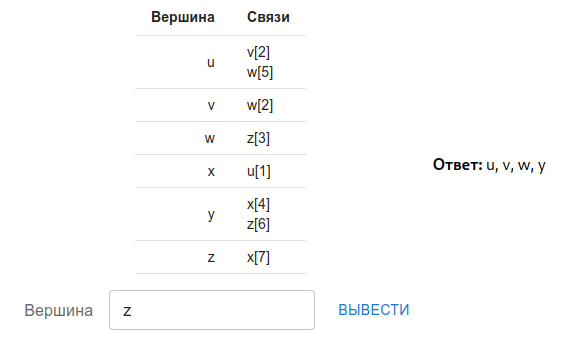
\includegraphics[width=0.8\textwidth]{figs/task-3/res-2.png}
  \caption{Результат работы}
\end{figure}
\section{Список смежности Iб: несколько графов}
\subsection{Условие задания}
\textbf{Вариант 8:} Построить орграф, являющийся пересечением двух заданных.

\subsection{Примеры исходного кода}
Для нахождения пересечения двух орграфов был описан метод \mitext{intersect()}:
\begin{minted}{typescript}
intersect(other: Graph): Graph {
  if (!this.oriented || !other.oriented) {
    throw new InvalidOperandTypes()
  }

  const res = new Graph(this.weighted || other.weighted, true)
  const intersection = new Map<string, Map<string, number>>()

  const commonNodes = Array.from(this.adj.keys()).filter(node => other.adj.has(node))

  for (const node of commonNodes) {
    const neighborsA = this.adj.get(node) || new Map<string, number>()
    const neighborsB = other.adj.get(node) || new Map<string, number>()
    const commonNeighbors = new Map<string, number>()

    for (const [neighbor, weightA] of neighborsA) {
      if (neighborsB.has(neighbor)) {
        const weightB = neighborsB.get(neighbor) || 0
        commonNeighbors.set(neighbor, Math.min(weightA, weightB))
      }
    }

    intersection.set(node, commonNeighbors)
  }

  res.adj = intersection
  return res
}
\end{minted}

В интерфейсе орграф"=пересечение выводится как обычно, в виде списка смежности.

\subsection{Краткое описание алгоритма}
Создается новый граф, в котором будет накапливаться результат. Затем
по определению "--- добавляем в результат только нужные вершины и дуги.

\subsection{Примеры входных и выходных данных}
\subsubsection{Входные данные}
\begin{figure}[H]
  \begin{minipage}{0.5\textwidth}
    \centering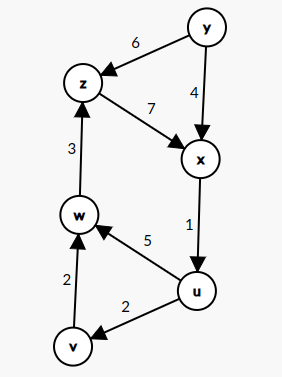
\includegraphics[width=0.6\linewidth]{figs/task-4/graph-3.png}
  \end{minipage}
  \begin{minipage}{0.5\textwidth}
    \centering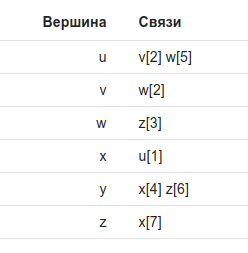
\includegraphics[width=0.6\linewidth]{figs/task-4/adj-3.png}
  \end{minipage}
  \caption{Первый ориентированный граф}
\end{figure}

\begin{figure}[H]
  \begin{minipage}{0.5\textwidth}
    \centering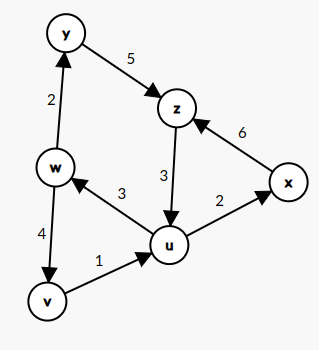
\includegraphics[width=0.6\linewidth]{figs/task-4/graph-4.png}
  \end{minipage}
  \begin{minipage}{0.5\textwidth}
    \centering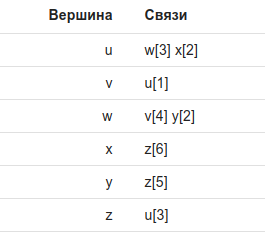
\includegraphics[width=0.6\linewidth]{figs/task-4/adj-4.png}
  \end{minipage}
  \caption{Второй ориентированный граф}
\end{figure}

\begin{minipage}{0.5\textwidth}
  \begin{minted}{js}
// первый орграф
{
  "weighted": true,
  "oriented": true,
  "adj": {
    "u": {
      "w": 3,
      "x": 2
    },
    "v": {
      "u": 1
    },
    "w": {
      "v": 4,
      "y": 2
    },
    "x": {
      "z": 6
    },
    "y": {
      "z": 5
    },
    "z": {
      "u": 3
    }
  }
}
  \end{minted}
\end{minipage}
\begin{minipage}{0.5\textwidth}
  \begin{minted}{js}
// второй орграф
{
  "weighted": true,
  "oriented": true,
  "adj": {
    "u": {
      "v": 2,
      "w": 5
    },
    "v": {
      "w": 2
    },
    "w": {
      "z": 3
    },
    "x": {
      "u": 1
    },
    "y": {
      "x": 4,
      "z": 6
    },
    "z": {
      "x": 7
    }
  }
}
  \end{minted}
\end{minipage}

\subsubsection{Выходные данные}
\begin{figure}[H]
  \begin{minipage}{0.5\textwidth}
    \centering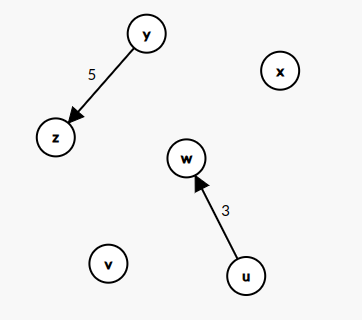
\includegraphics[width=0.8\linewidth]{figs/task-4/res-graph-4.png}
  \end{minipage}
  \begin{minipage}{0.5\textwidth}
    \centering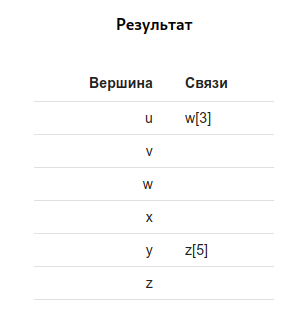
\includegraphics[width=0.8\linewidth]{figs/task-4/res-4.png}
  \end{minipage}
  \caption{Результат работы}
\end{figure}
\section{Обходы графа II}
\subsection{Условие задания}
\textbf{Вариант 5:} Подсчитать количество связных компонент графа.

\subsection{Примеры исходного кода}
Для нахождения компонент связности графа был описан метод\\
\mitext{connectedComponents()}:
\begin{minted}{typescript}
connectedComponents(): number {
  const visited: Set<string> = new Set()

  let count = 0 // количество компонент
  for (const node of this.adj.keys()) {
    if (!visited.has(node)) { // если еще не посетили, выполнить DFS
      count++ // новая компонента
      this.dfs(node, visited) // DFS посещаем все узлы в этой компоненте связности
    }
  }

  return count
}
\end{minted}

А также вспомогательный метод обхода в глубину:
\begin{minted}{typescript}
private dfs(node: string, visited: Set<string>) {
  visited.add(node)

  const neighbors = this.adj.get(node)!
  for (const neighbor of neighbors.keys()) {
    if (!visited.has(neighbor)) {
      this.dfs(neighbor, visited) // рекурсивно обойти соседние узлы
    }
  }
}
\end{minted}

\subsection{Краткое описание алгоритма}
Вводится счетчик количества компонент связности. Также ведется множество
уже посещенных вершин. Алгоритм заканчивает работу, когда все вершины посещены.
На каждой итерации выбирается непосещенная вершина и с помощью обхода
в глубину посещаются все связные с ней вершины (одна компонента связности).
Таким образом, мы сможем подсчитать, сколько всего компонент связности
в графе.

\subsection{Примеры входных и выходных данных}
\subsubsection{Входные данные}
\begin{figure}[H]
  \begin{minipage}{0.5\textwidth}
    \centering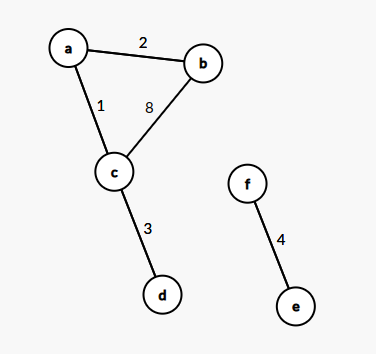
\includegraphics[width=0.6\linewidth]{figs/task-5/graph-5.png}
  \end{minipage}
  \begin{minipage}{0.5\textwidth}
    \centering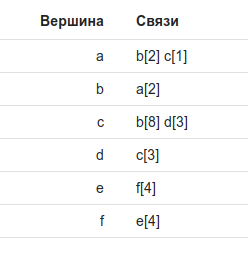
\includegraphics[width=0.6\linewidth]{figs/task-5/adj-5.png}
  \end{minipage}
  \caption{Неориентированный граф}
\end{figure}

\begin{minted}{js}
{
  "weighted": true,
  "oriented": false,
  "adj": {
    "a": {
      "b": 2,
      "c": 1
    },
    "b": {
      "a": 2
    },
    "c": {
      "a": 1,
      "d": 3
    },
    "d": {
      "c": 3
    },
    "e": {
      "f": 4
    },
    "f": {
      "e": 4
    }
  }
}
\end{minted}

\subsubsection{Выходные данные}
\begin{figure}[H]
  \centering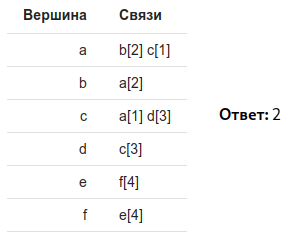
\includegraphics[width=0.4\textwidth]{figs/task-5/res-5.png}
  \caption{Результат работы}
\end{figure}
\section{Обходы графа II}
\subsection{Условие задания}
\textbf{Вариант 27:} Найти длины кратчайших (по числу дуг) путей из вершины $u$ во все остальные.

\subsection{Примеры исходного кода}
Для нахождения длины кратчайших путей из вершины $u$ во все остальные
был объявлен метод \mitext{shortestPathLengthsFrom()}, принимающий
метку вершины $u$ и возвращающий расстояния до всех вершин графа (по числу дуг):
\begin{minted}{typescript}
shortestPathLengthsFrom(u: string): Map<string, number> {
  if (!this.adj.has(u)) {
    throw new NodeNotExists(u)
  }

  const shortestPaths: Map<string, number> = new Map()

  for (const node of this.adj.keys()) {
    shortestPaths.set(node, Infinity) // пока считаем, что расстояния до других узлов бесконечность
  }
  shortestPaths.set(u, 0) // расстояние до самого себя 0

  const queue = [u] // очередь обхода
  while (queue.length > 0) {
    const currentNode = queue.shift()!
    const neighbors = this.adj.get(currentNode)!

    for (const neighbor of neighbors.keys()) {
      if (shortestPaths.get(neighbor) === Infinity) { // если узел еще не был посещен
        // установить кратчайшее расстояние до него
        shortestPaths.set(neighbor, shortestPaths.get(currentNode)! + 1)
        queue.push(neighbor) // добавить соседний узел в очередь обхода
      }
    }
  }

  return shortestPaths
}
\end{minted}

\subsection{Краткое описание алгоритма}
Этот алгоритм использует метод обхода в ширину (BFS) для нахождения кратчайших путей.

Создается \mitext{Map<string, number>}, где для каждой вершины устанавливается начальное расстояние.
Расстояние от $u$ до самой себя равно $0$, а до остальных вершин "--- бесконечность.

Используется очередь для обхода графа. Начальная вершина $u$ добавляется в очередь.
Пока очередь не пуста, извлекается текущая вершина. Для каждого соседнего узла проверяется,
был ли он уже посещен. Если не был, устанавливается кратчайшее расстояние и добавляется в очередь.

\subsection{Примеры входных и выходных данных}
\subsubsection{Входные данные}
\begin{figure}[H]
  \begin{minipage}{0.5\textwidth}
    \centering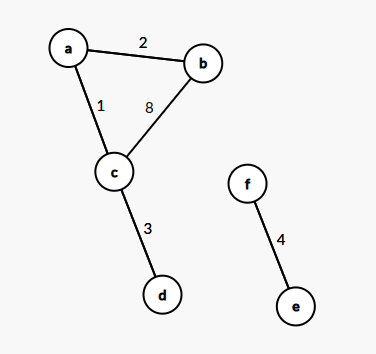
\includegraphics[width=0.6\linewidth]{figs/task-6/graph-6.png}
  \end{minipage}
  \begin{minipage}{0.5\textwidth}
    \centering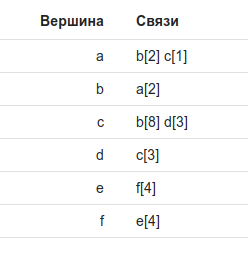
\includegraphics[width=0.6\linewidth]{figs/task-6/adj-6.png}
  \end{minipage}
  \caption{Неориентированный граф}
\end{figure}

\begin{minted}{js}
{
  "weighted": true,
  "oriented": false,
  "adj": {
    "a": {
      "b": 2,
      "c": 1
    },
    "b": {
      "a": 2
    },
    "c": {
      "a": 1,
      "d": 3
    },
    "d": {
      "c": 3
    },
    "e": {
      "f": 4
    },
    "f": {
      "e": 4
    }
  }
}
\end{minted}

\subsubsection{Выходные данные}
\begin{figure}[H]
  \centering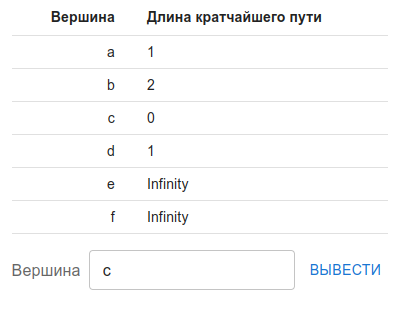
\includegraphics[width=0.4\textwidth]{figs/task-6/res-6.png}
  \caption{Результат работы}
\end{figure}
\section{Каркас III}
\subsection{Условие задания}
Дан взвешенный неориентированный граф из $N$ вершин и $M$ ребер.
Требуется найти в нем каркас минимального веса. (Алгоритм Прима)

\subsection{Примеры исходного кода}
Для нахождения каркаса минимального веса взвешенного неориентированного
графа был создан метод \mitext{mst()} (\textit{Minimal Spanning Tree}):
\begin{minted}{typescript}
mst(): Graph {
  if (!this.weighted || this.oriented) {
    throw new GraphNotWeightedUnoriented()
  }

  const mst = new Graph(true, false) // минимальное остовное дерево
  const visited = new Set<string>() // множество посещенных вершин

  // взять любую вершину как начальную (здесь первая)
  const startVertex = this.adj.keys().next().value
  if (!startVertex) {
    throw new GraphIsEmpty()
  }
  visited.add(startVertex)
  mst.addNode(startVertex)

  while (visited.size < this.adj.size) { // пока не посетим все вершины
    // ребра, которые соединяют посещенные вершины с непосещенными
    const edges: Array<Edge> = []

    for (const vertex of visited) { // найти такие ребра
      for (const [neighbor, weight] of this.adj.get(vertex)!) {
        if (!visited.has(neighbor)) {
          edges.push({from: vertex, to: neighbor, weight});
        }
      }
    }

    if (edges.length === 0) {
      // Не все вершины еще посещены, но мы не смогли найти новые ребра.
      // Это значит, что граф несвязный.
      throw new GraphIsNotConnected()
    }

    // выбрать ребро с наименьшим весом
    edges.sort((a, b) => a.weight - b.weight)
    const {from, to, weight} = edges[0]

    // добавить ребро в минимальное остовное дерево
    mst.addNode(to)
    mst.connect(from, to, weight)
    visited.add(to)
  }

  return mst
}
\end{minted}

\subsection{Краткое описание алгоритма}
Основная идея заключается в том, чтобы начать с одной вершины и пошагово добавлять ребра
минимального веса, соединяющие посещенные вершины с непосещенными.

Создается новый граф \mitext{mst}, представляющий минимальное остовное дерево.
Также создается множество \mitext{visited} для отслеживания посещенных вершин.
Выбирается любая вершина в качестве начальной. В данной реализации используется
первая вершина из списка вершин графа.

Пока не посещены все вершины графа, выполняется цикл:
\begin{enumerate}
  \item Создается массив \mitext{edges}, содержащий ребра, соединяющие посещенные вершины с непосещенными.
  \item Если массив \mitext{edges} пуст, это означает, что граф несвязный (ошибка).
  \item Ребра в массиве сортируются по весу, и выбирается ребро с минимальным весом.
  \item Выбранное ребро добавляется в остовное дерево, связывая вершины \mitext{from} и \mitext{to} с весом
  \mitext{weight}. Вершина \mitext{to} помечается как посещенная.
\end{enumerate}

\subsection{Примеры входных и выходных данных}
\subsubsection{Входные данные}
\begin{figure}[H]
  \begin{minipage}{0.5\textwidth}
    \centering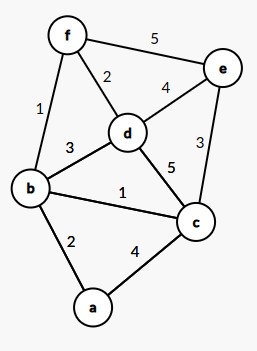
\includegraphics[width=0.6\linewidth]{figs/task-7/graph-7.png}
  \end{minipage}
  \begin{minipage}{0.5\textwidth}
    \centering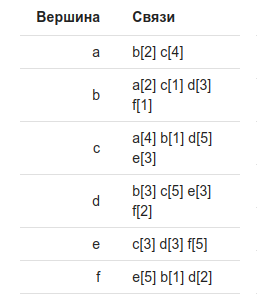
\includegraphics[width=0.6\linewidth]{figs/task-7/adj-7.png}
  \end{minipage}
  \caption{Неориентированный взвешенный граф}
\end{figure}

\begin{minted}{js}
{
  "weighted": true,
  "oriented": false,
  "adj": {
    "a": {
      "b": 2,
      "c": 4
    },
    "b": {
      "a": 2,
      "c": 1,
      "d": 3,
      "f": 1
    },
    "c": {
      "a": 4,
      "b": 1,
      "d": 5,
      "e": 3
    },
    "d": {
      "b": 3,
      "c": 5,
      "e": 3,
      "f": 2
    },
    "e": {
      "c": 3,
      "d": 4,
      "f": 5
    },
    "f": {
      "e": 5,
      "b": 1,
      "d": 2
    }
  }
}
\end{minted}

\subsubsection{Выходные данные}
\begin{figure}[H]
  \begin{minipage}{0.5\textwidth}
    \centering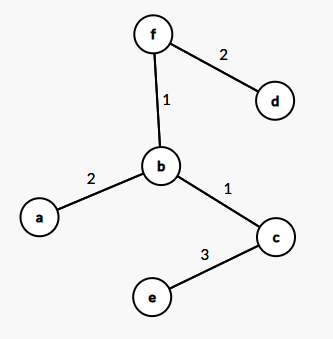
\includegraphics[width=0.8\linewidth]{figs/task-7/res-graph-7.png}
  \end{minipage}
  \begin{minipage}{0.5\textwidth}
    \centering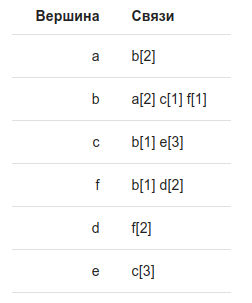
\includegraphics[width=0.6\linewidth]{figs/task-7/res-7.png}
  \end{minipage}
  \caption{Результат работы}
\end{figure}

\conclusion
В ходе практики был выполнен ряд задач, которые поспособствовали закреплению
и углублению теоретических знаний по дисциплине <<Теория графов>>, посредством
реализации класса <<Граф>> на языке TypeScript.

\inputencoding{cp1251}
\bibliographystyle{gost780uv}
\bibliography{thesis}
\inputencoding{utf8}

% Окончание основного документа и начало приложений Каждая последующая секция
% документа будет являться приложением
\appendix
\section{Компонент \mitext{App} веб"=интерфейса}
\label{app:app-component}

\begin{minted}{jsx}
function App() {
  const graph = useRef(new Graph(false, false))
  const [newNode, setNewNode] = useState<string>('')
  const [deleteNode, setDeleteNode] = useState<string>('')
  const [connNodeA, setConnNodeA] = useState<string>('')
  const [connNodeB, setConnNodeB] = useState<string>('')
  const [connNodeWeight, setConnNodeWeight] = useState<number | null>(null)
  const [delConnA, setDelConnA] = useState<string>('')
  const [delConnB, setDelConnB] = useState<string>('')
  const [shouldRerender, setShouldRerender] = useState<boolean>(true)

  const orientedSelection = useRef('unoriented')
  const weightedSelection = useRef('non-weighted')

  useEffect(() => {
      setShouldRerender(false)
    }, [shouldRerender]
  )

  function onCreateNodeClick() {
    if (!newNode) {
      alert('Незаполненные поля!')
      return
    }

    try {
      graph.current.addNode(newNode)
    }
    catch (e) {
      if (e instanceof GraphError) {
        alert(e.message)
        return
      }
    }
    setNewNode('')
    setShouldRerender(true)
  }

  function onDeleteNodeClick() {
    if (!deleteNode) {
      alert('Незаполненные поля!')
      return
    }

    try {
      graph.current.removeNode(deleteNode)
    }
    catch (e) {
      if (e instanceof GraphError) {
        alert(e.message)
        return
      }
    }
    setDeleteNode('')
    setShouldRerender(true)
  }

  function onConnectNodesClick() {
    if (!connNodeA || !connNodeB || (graph.current.isWeighted() && !connNodeWeight)) {
      alert('Незаполненные поля!')
      return
    }

    try {
      graph.current.connect(connNodeA, connNodeB, connNodeWeight ?? undefined)
    }
    catch (e) {
      if (e instanceof GraphError) {
        alert(e.message)
        return
      }
    }
    setConnNodeA('')
    setConnNodeB('')
    setConnNodeWeight(null)
    setShouldRerender(true)
  }

  function onDeleteConnectionClick() {
    if (!delConnA || !delConnB) {
      alert('Незаполненные поля!')
      return
    }

    try {
      graph.current.disconnect(delConnA, delConnB)
    }
    catch (e) {
      if (e instanceof GraphError) {
        alert(e.message)
        return
      }
    }
    setDelConnA('')
    setDelConnB('')
    setShouldRerender(true)
  }

  function onGraphLoaded(fileContent: string) {
    try {
      graph.current = new Graph(fileContent)
    }
    catch (e) {
      alert('Неверный формат файла!')
      return
    }

    if (graph.current.isOriented()) {
      orientedSelection.current = 'oriented'
    }
    else {
      orientedSelection.current = 'unoriented'
    }

    if (graph.current.isWeighted()) {
      weightedSelection.current = 'weighted'
    }
    else {
      weightedSelection.current = 'non-weighted'
    }

    setShouldRerender(true)
  }

  function onGraphOrientedChange(value: string) {
    orientedSelection.current = value
    graph.current.changeOriented(value === 'oriented')
    setShouldRerender(true)
  }

  function onGraphWeightedChange(value: string) {
    weightedSelection.current = value
    graph.current.changeWeighted(value === 'weighted')
    setShouldRerender(true)
  }

  return (
    <div id='app'>
      <header>
        <h2>Взаимодействие с графом</h2>
      </header>
      <div className='controls'>
        <div className='control' style={{ gridColumnStart: '2', gridColumnEnd: '4' }}>
          <InputLabel>Ориентированность</InputLabel>
          <Select value={orientedSelection.current}
                  onChange={e => onGraphOrientedChange(e.target.value)}>
            <MenuItem value='unoriented'>Неориентированный</MenuItem>
            <MenuItem value='oriented'>Ориентированный</MenuItem>
          </Select>
        </div>
        <div className='control' style={{ gridColumnStart: '4', gridColumnEnd: '6' }}>
          <InputLabel>Взвешенность</InputLabel>
          <Select value={weightedSelection.current}
                  onChange={e => onGraphWeightedChange(e.target.value)}>
            <MenuItem value='weighted'>Взвешенный</MenuItem>
            <MenuItem value='non-weighted'>Невзвешенный</MenuItem>
          </Select>
        </div>
        <div className='control' style={{gridTemplateColumns: '1fr 1fr 1fr', gridColumnStart: '2', gridColumnEnd: '6'}}>
          <GraphLoader onGraphLoaded={onGraphLoaded} />
          <GraphDumper graph={graph} />
        </div>
        <div className='control' style={{gridColumnStart: '2', gridColumnEnd: '4'}}>
          <InputLabel>Создать узел</InputLabel>
          <TextField value={newNode ?? ''}
                     type='text'
                     onChange={e => setNewNode(e.target.value)}
                     size='small'>
          </TextField>
          <Button onClick={onCreateNodeClick}>Добавить</Button>
        </div>
        <div className='control' style={{gridColumnStart: '4', gridColumnEnd: '6'}}>
          <InputLabel>Удалить узел</InputLabel>
          <TextField value={deleteNode ?? ''}
                     type='text'
                     onChange={e => setDeleteNode(e.target.value)}
                     size='small'>
          </TextField>
          <Button onClick={onDeleteNodeClick}>Удалить</Button>
        </div>
        <div className='control' style={{gridColumnStart: '2', gridColumnEnd: '4'}}>
          <InputLabel>Соединить узлы</InputLabel>
          <div style={{ display: 'grid', gridTemplateRows: '1fr 1fr 1fr'}}>
            <TextField value={connNodeA ?? ''}
                       type='text'
                       onChange={e => setConnNodeA(e.target.value)}
                       size='small'
                       style={{paddingBottom: '0.5em'}}>
            </TextField>
            <TextField value={connNodeB ?? ''}
                       type='text'
                       onChange={e => setConnNodeB(e.target.value)}
                       size='small'
                       style={{paddingBottom: '0.5em'}}>
            </TextField>
            <TextField value={connNodeWeight ?? ''}
                       type='number'
                       onChange={e => setConnNodeWeight(Number(e.target.value))}
                       size='small'>
            </TextField>
          </div>
          <Button onClick={onConnectNodesClick}>Соединить</Button>
        </div>
        <div className='control' style={{gridColumnStart: '4', gridColumnEnd: '6'}}>
          <InputLabel>Удалить связь</InputLabel>
          <div style={{ display: 'grid', gridTemplateRows: '1fr 1fr'}}>
            <TextField value={delConnA ?? ''}
                       type='text'
                       onChange={e => setDelConnA(e.target.value)}
                       size='small'
                       style={{paddingBottom: '0.5em'}}>
            </TextField>
            <TextField value={delConnB ?? ''}
                       type='text'
                       onChange={e => setDelConnB(e.target.value)}
                       size='small'>
            </TextField>
          </div>
          <Button onClick={onDeleteConnectionClick}>Удалить</Button>
        </div>
      </div>
      <main style={{width: '100%', display: 'flex', justifyContent: 'center'}}>
        <div id='connections'>
          <GraphView graph={graph} />
        </div>
      </main>
      <hr />
      <div id='tasks'>
        <TaskOne />
        <hr />
        <!-- Остальные компоненты задач -->
      </div>
    </div>
  )
}
\end{minted}

\end{document}